\chapter{Beam Dynamics in Rings}
\label{sec:ch2}

\section{\label{sec:lie}Lie Maps in Accelerator Physics}

The most basic element of a particle accelerator can be thought of as a black box. This black box takes some single charged particle with initial transverse coordinates $\left( x_0,x'_0,y_0,y'_0 \right)$, as defined in a Frenet-Serret coordinate system, and maps them to some final coordinates $\left( x_f,x'_f,y_f,y'_f \right)$. For simplicity, any longitudinal effect will not be taken into account for this analysis, but can be easily incorporated. By gathering the initial coordinates into a vector, i.e. $\vec{X_0} = \left( x_0,x_0',y_0,y_0' \right)$, and doing the same for the final coordinates, i.e., $\vec{X_f} = \left( x_f,x_f',y_f,y_f' \right)$, one can define the mapping $\mathcal{M}$ that relates both vectors, such that:  
\begin{equation}
\label{eq:ch2map}
\vec{X_f}=\mathcal{M}\vec{X_0}.
\end{equation}
For a charged particle inside some accelerator element that can be described using Hamiltonian dynamics, the mapping $\mathcal{M}$ can be understood in terms of Poisson brackets and exponential Lie operators \cite{wolski,todd1,cernthesis1,cernthesis2}.\\
Let $\vec{X} = \left( q_1,p_1,\dots,q_{n},p_{n} \right)$ be a 2n dimensional vector, made from $n$ pairs of canonical coordinates $(q_i,p_i)$ that make up the 2$n$ dimensional phase space. And let two arbitrary functions $f\left( \vec{X};s\right)$ and $g\left( \vec{X};s\right)$ be functions of $\vec{X}$ and $s$, where $s$ plays the role of the independent "time" coordinate. The Poisson brackets $\left[ \bullet , \bullet \right]$ can be defined as:
\begin{equation}
    \label{eq:ch2poisson}
    \left[ f,g \right] = \sum_{i=1}^{n} \frac{\partial f}{\partial q_i}\frac{\partial g}{\partial p_i} - \frac{\partial f}{\partial p_i}\frac{\partial g}{\partial q_i}. 
\end{equation}
Using this definition, one can explicitly write out the Poisson bracket definition for a 4 dimensional phase space described by state vector $\vec{X} = \left( x,x',y,y' \right)$. This reads: 
\begin{equation}
    \label{eq:ch2poisson1}
    \left[ f,g \right] = \frac{\partial f}{\partial x}\frac{\partial g}{\partial x'} - \frac{\partial f}{\partial x'}\frac{\partial g}{\partial x} + \frac{\partial f}{\partial y}\frac{\partial g}{\partial y'} - \frac{\partial f}{\partial y'}\frac{\partial g}{\partial y}. 
\end{equation}\\
The Lie operator $:f:$ acts on some function $g$ and is the adjoint operator of the Poisson bracket operator. Its definition reads:
\begin{equation}
    \label{eq:ch2lie1}
    :f:g = \left[ f,g \right].
\end{equation}
This specific $:\bullet:$ notation allows for a compact notation in order to define the exponential Lie operator. The exponential Lie operator of an arbitrary function $f$ is defined as
\begin{equation}
    \label{eq:ch2explie1}
    e^{:f:}\bullet = \sum_{k=0}^{\infty}\frac{1}{k!}\left( :f: \right)^k \bullet.
\end{equation}
It turns out that for a Hamiltonian system, the mapping of coordinates from $\vec{X_0}$ to $\vec{X_f}$ follows the expression:
\begin{equation}
    \label{eq:ch2liemap1}
    \vec{X_f}=e^{-\ell :H:}\vec{X}\bigg\rvert_{\vec{X}=\vec{X_0}},
\end{equation}
which is known as a Lie Map \cite{todd1}. In this case, $\ell$ corresponds to the integration length of the independent coordinate. For example, for a particle traversing a magnet which has length $L$, the integration length is $\ell = L$. When looking at the one-turn map, the integration length corresponds to the circumference $C$ of the accelerator over an effective Hamiltonian $H_{eff}$. Furthermore, if working with action-angle variables, the integration length $\ell$ would just be the phase advance $\mu$.\\ 

\section{\label{sec:oneturn}One-turn Map and Normal Form}

The one-turn map $\mathcal{M}_1$ of a circular accelerator is the composition ($\circ$) of mappings from every element in the ring. Choosing an arbitrary initial point at $s=0$ and going around the ring, the one-turn map describes the transformation of coordinates after one turn, i.e., $\vec{X}_{N=1}=\mathcal{M}_1 \vec{X_0}$. This map composition reads:
\begin{equation}
    \label{eq:oneturnmap}
    \mathcal{M}_1=M_{N+1} \circ e^{:h_N:} \circ \dots \circ e^{:h_2:} \circ M_2 \circ e^{:h_1:} \circ M_1 = M_{N+1}e^{:h_N:} \dots e^{:h_2:}M_2 e^{:h_1:}M_1,
\end{equation}
where $M_i$ is the matrix representation of a linear mapping, that does not couple $x-y$ plane, e.g., drift space mapping, quadrupole mapping. On the other hand, the map $e^{:h_i:}$ represents any linear or non-linear mapping that can be found around the machine and can be considered a perturbation to the ideal lattice including coupling elements, e.g., skew quadrupoles, higher order multipole elements. Figure \ref{fig:oneturn} illustrates the procedure to build the one-turn map for a circular accelerator. 

\begin{figure}[H]
    \centering
    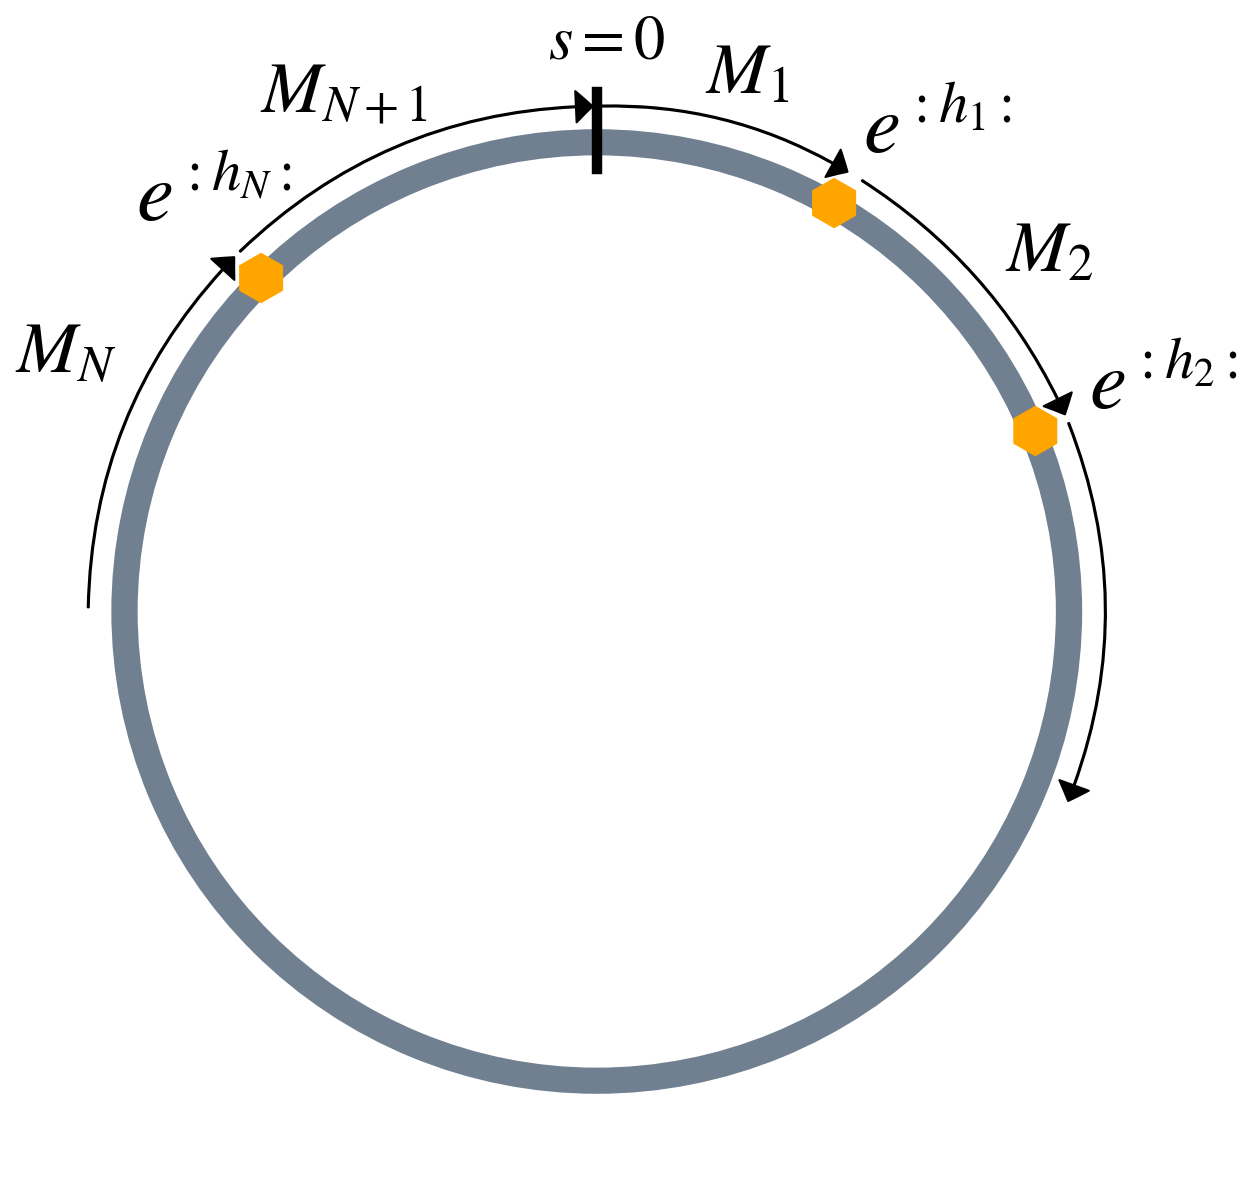
\includegraphics[width=0.7\columnwidth]{chapter2/oneturn.png}
    \caption{Diagram of an arbitrary circular accelerator in order to illustrate the one-turn map.}
    \label{fig:oneturn}
 \end{figure}

Through the use of the Baker-Campbell-Hausdorff formula , Eq. \ref{eq:oneturnmap} can be collapsed to the expression 
\begin{equation}
    \label{eq:oneturnmapeff}
    \mathcal{M}_1=e^{-C :H_{eff}:},
\end{equation}
where $C$ is the circumference of the ring and $H_{eff}$ is the effective Hamiltonian of the machine over one turn. As mentioned earlier, for most cases, it is of interest to look at the perturbations to the linear uncoupled dynamics of the design lattice. With this in mind, Eq. \ref{eq:oneturnmapeff} can be rewritten as:
\begin{equation}
    \label{eq:oneturnmapeff1}
    \mathcal{M}_1=e^{:h:}R,
\end{equation}
where $R$ is a rotation matrix encoding the linear uncoupled dynamics of the ideal lattice. On the other hand, the term $e^{:h:}$ encodes the perturbations to this ideal situation. It is worth pointing out that for the case $h=0$, the traditional Courant-Snyder variables are recovered.   

The Courant-Snyder variables ($\hat{x}$,$\hat{p}_x$,$\hat{y}$,$\hat{p}_y$) or normalized phase space coordinates can be written for a linear uncoupled case as:
\begin{equation}
    \label{eq:norm1}
    \hat{u}=\sqrt{2J_u} \cos \left( \phi_u + \phi_{u_0}\right);
\end{equation}
\begin{equation}
    \label{eq:norm2}
    \hat{p}_u=-\sqrt{2J_u} \sin \left( \phi_u + \phi_{u_0}\right),
\end{equation}
where $u$ can stand either for the $x$ or $y$ coordinate, $J_u$ and $\phi_u$ correspond to the action-angle variables and $\phi_{u_0}$ corresponds to the initial phase. For the case where perturbations exist, i.e., $h \neq 0$, the action $J_u$ is not constant anymore and will be a function of $\phi_u$.  

The Normal Form formalism is introduced at this point in order to find amplitude-independent coordinates $I_u$ and $\psi_u$, such that the motion just depends on $\psi_u$ at a constant $I_u$, with some initial phase $\psi_{u_0}$. These are known as non-linear action-angle variables. The variables $I_u$ and $\psi_u$ are calculated from the transformation $e^{-:F:}$ acting on $J_u$ and $\phi_u$. Without loss of generality, the generating function $F$ can be written as a Fourier expansion over the objective space $(I_x,\psi_x,I_y,\psi_y)$ such that:
\begin{equation}
    \label{eq:F}
    F=\sum_{jklm} f_{jklm} \left( 2 I_x\right)^{\frac{j+k}{2}} \left( 2 I_y\right)^{\frac{l+m}{2}} e^{i\left[ \left( j-k \right)\left( \psi_x+\psi_{x0} \right)+ \left( l-m \right) \left( \psi_y+\psi_{y0} \right)\right]}.
\end{equation}
In a similar fashion, the argument of the Lie operator $e^{:h:}$ from Eq. \ref{eq:oneturnmapeff1} can be expanded as:
\begin{equation}
    \label{eq:h}
    h=\sum_{jklm} h_{jklm} \left( 2 J_x\right)^{\frac{j+k}{2}} \left( 2 J_y\right)^{\frac{l+m}{2}} e^{i\left[ \left( j-k \right)\left( \phi_x+\phi_{x0} \right)+ \left( l-m \right) \left( \phi_y+\phi_{y0} \right)\right]}.
\end{equation}
For Eqs. \ref{eq:F} and \ref{eq:h}, the integer indices $j,k,l,m$ run from $0$ to infinity, and correspond to the four degrees of freedom for transverse phase space.   

The terms $f_{jklm}$ are known as generating function coefficients. The terms $h_{jklm}$ are known as Hamiltonian coefficients or resonance driving terms (RDTs). Section \ref{sec:rdts} will take a closer look into how RDTs can be used to characterize the non-linear dynamics of accelerators. The generating function coefficients $f_{jklm}$ can be related to the Hamiltonian resonance driving terms $h_{jklm}$ through the following relation \cite{cernthesis1,bartolini}:
\begin{equation}
    \label{eq:handf}
    f_{jklm}=\frac{h_{jklm}}{1-e^{2\pi i \left[ \left( j-k \right) Q_x + \left( l-m\right) Q_y \right] }},
\end{equation}
where $Q_x$ and $Q_y$ represent the transverse uncoupled and unperturbed tunes of the accelerator. The transverse tunes of a circular accelerator are defined as the phase advances in each plane over one turn, in units of $2\pi$, i.e., $Q_u=\phi_u(s=C)/2\pi$. 

\section{Resonances in Circular Accelerators}

Equation \ref{eq:handf} diverges for when the denominator goes to zero. Specifically, this happens when the following condition is met:
\begin{equation}
    \label{eq:resonances}
    \left( j-k \right) Q_x + \left( l-m\right) Q_y = p,
\end{equation}
where $p$ can be any integer. Equation \ref{eq:resonances} defines resonance lines in tune space of order $n=j+k+l+m$. If the accelerator is tuned to operate on top of these resonances, the perturbations will add up coherently turn to turn and kick the resonant particles out of their original trajectory. In general, operating close or on top of a resonance line is harmful as particles will be lost. This is specially true for lower order resonances, i.e., for $n<4$. In general, the higher order of a resonance, the weaker it is \cite{Wiedemann2015}. This thesis work focuses on third order resonances, i.e., $n=3$, and how to mitigate their deleterious effect. 

Figure \ref{fig:tunediagram} shows the tune diagram with resonance lines, as defined by Eq. \ref{eq:resonances}, drawn up to fifth order. The integer part of both tunes are chosen to include the actual area of operation of the Recycler Ring. Nevertheless, the fractional part of the tune carries the significant information for resonance diagrams. The operation and tune diagram for the Recycler Ring are described in more detail in Ch. \ref{sec:ch3}. Normally, the operation point of a circular accelerator is chosen to be clear of any resonance line and far away as possible from integer ($n=1$) and half integer ($n=2$) resonances. Nevertheless, in reality there are two concepts that complicate things. The first one relates to the fact that resonance lines are not infinitely thin and have some stop band width. The second one, concerns the fact that at high intensities particles will not have localized tunes, but rather a distribution of tunes with some tune spread, i.e., a tune footprint. Section \ref{sec:sc1} takes a closer look at this effect known as space charge tune shift. Ultimately, choosing the operation point on Fig. \ref{fig:tunediagram} is a matter of localizing a resonance-free region where the intensity-dependent tune footprint can be placed.   
\begin{figure}[H]
    \centering
    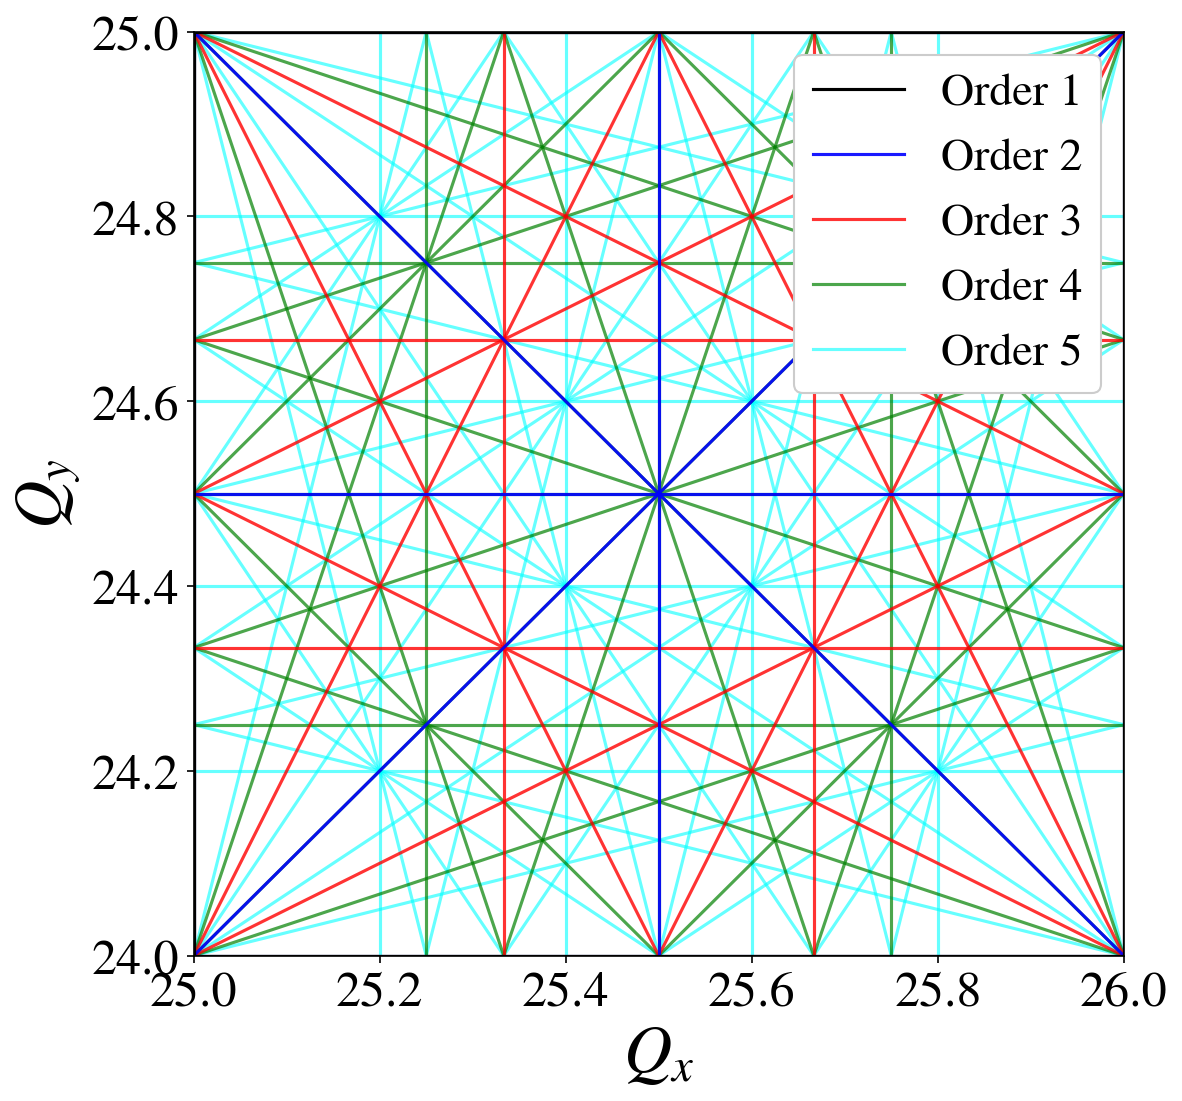
\includegraphics[width=0.8\columnwidth]{chapter2/tunediagram.png}
    \caption{Tune diagram with resonance lines up to fifth order, enclosing the operation point of the Recycler Ring.}
    \label{fig:tunediagram}
 \end{figure}
It is worth stopping here and asking what is the driving force behind each of these resonance lines. Classic accelerator references such as Refs. \cite{wolski,Wiedemann2015,sylee} will derive Eq. \ref{eq:resonances} by perturbing Hill's equation with different magnetic multipole orders. A closer look into each perturbation term reveals that half integer resonances are caused by quadrupole terms, third order resonances by sextupole-like terms, fourth order resonances by octupole terms, and so on and so forth. Nevertheless, the story complicates when one takes into account that pure multipole magnets can feed down to higher order terms, e.g., a tilted quadrupole feeds down to sextupole-like terms.        

Figure \ref{fig:rrtdlow} zooms into the region of interest for the Recycler Ring operation in the tune diagram, as shown in Fig. \ref{fig:tunediagram}. As mentioned before, the operation point   

 \begin{figure}[H]
    \centering
    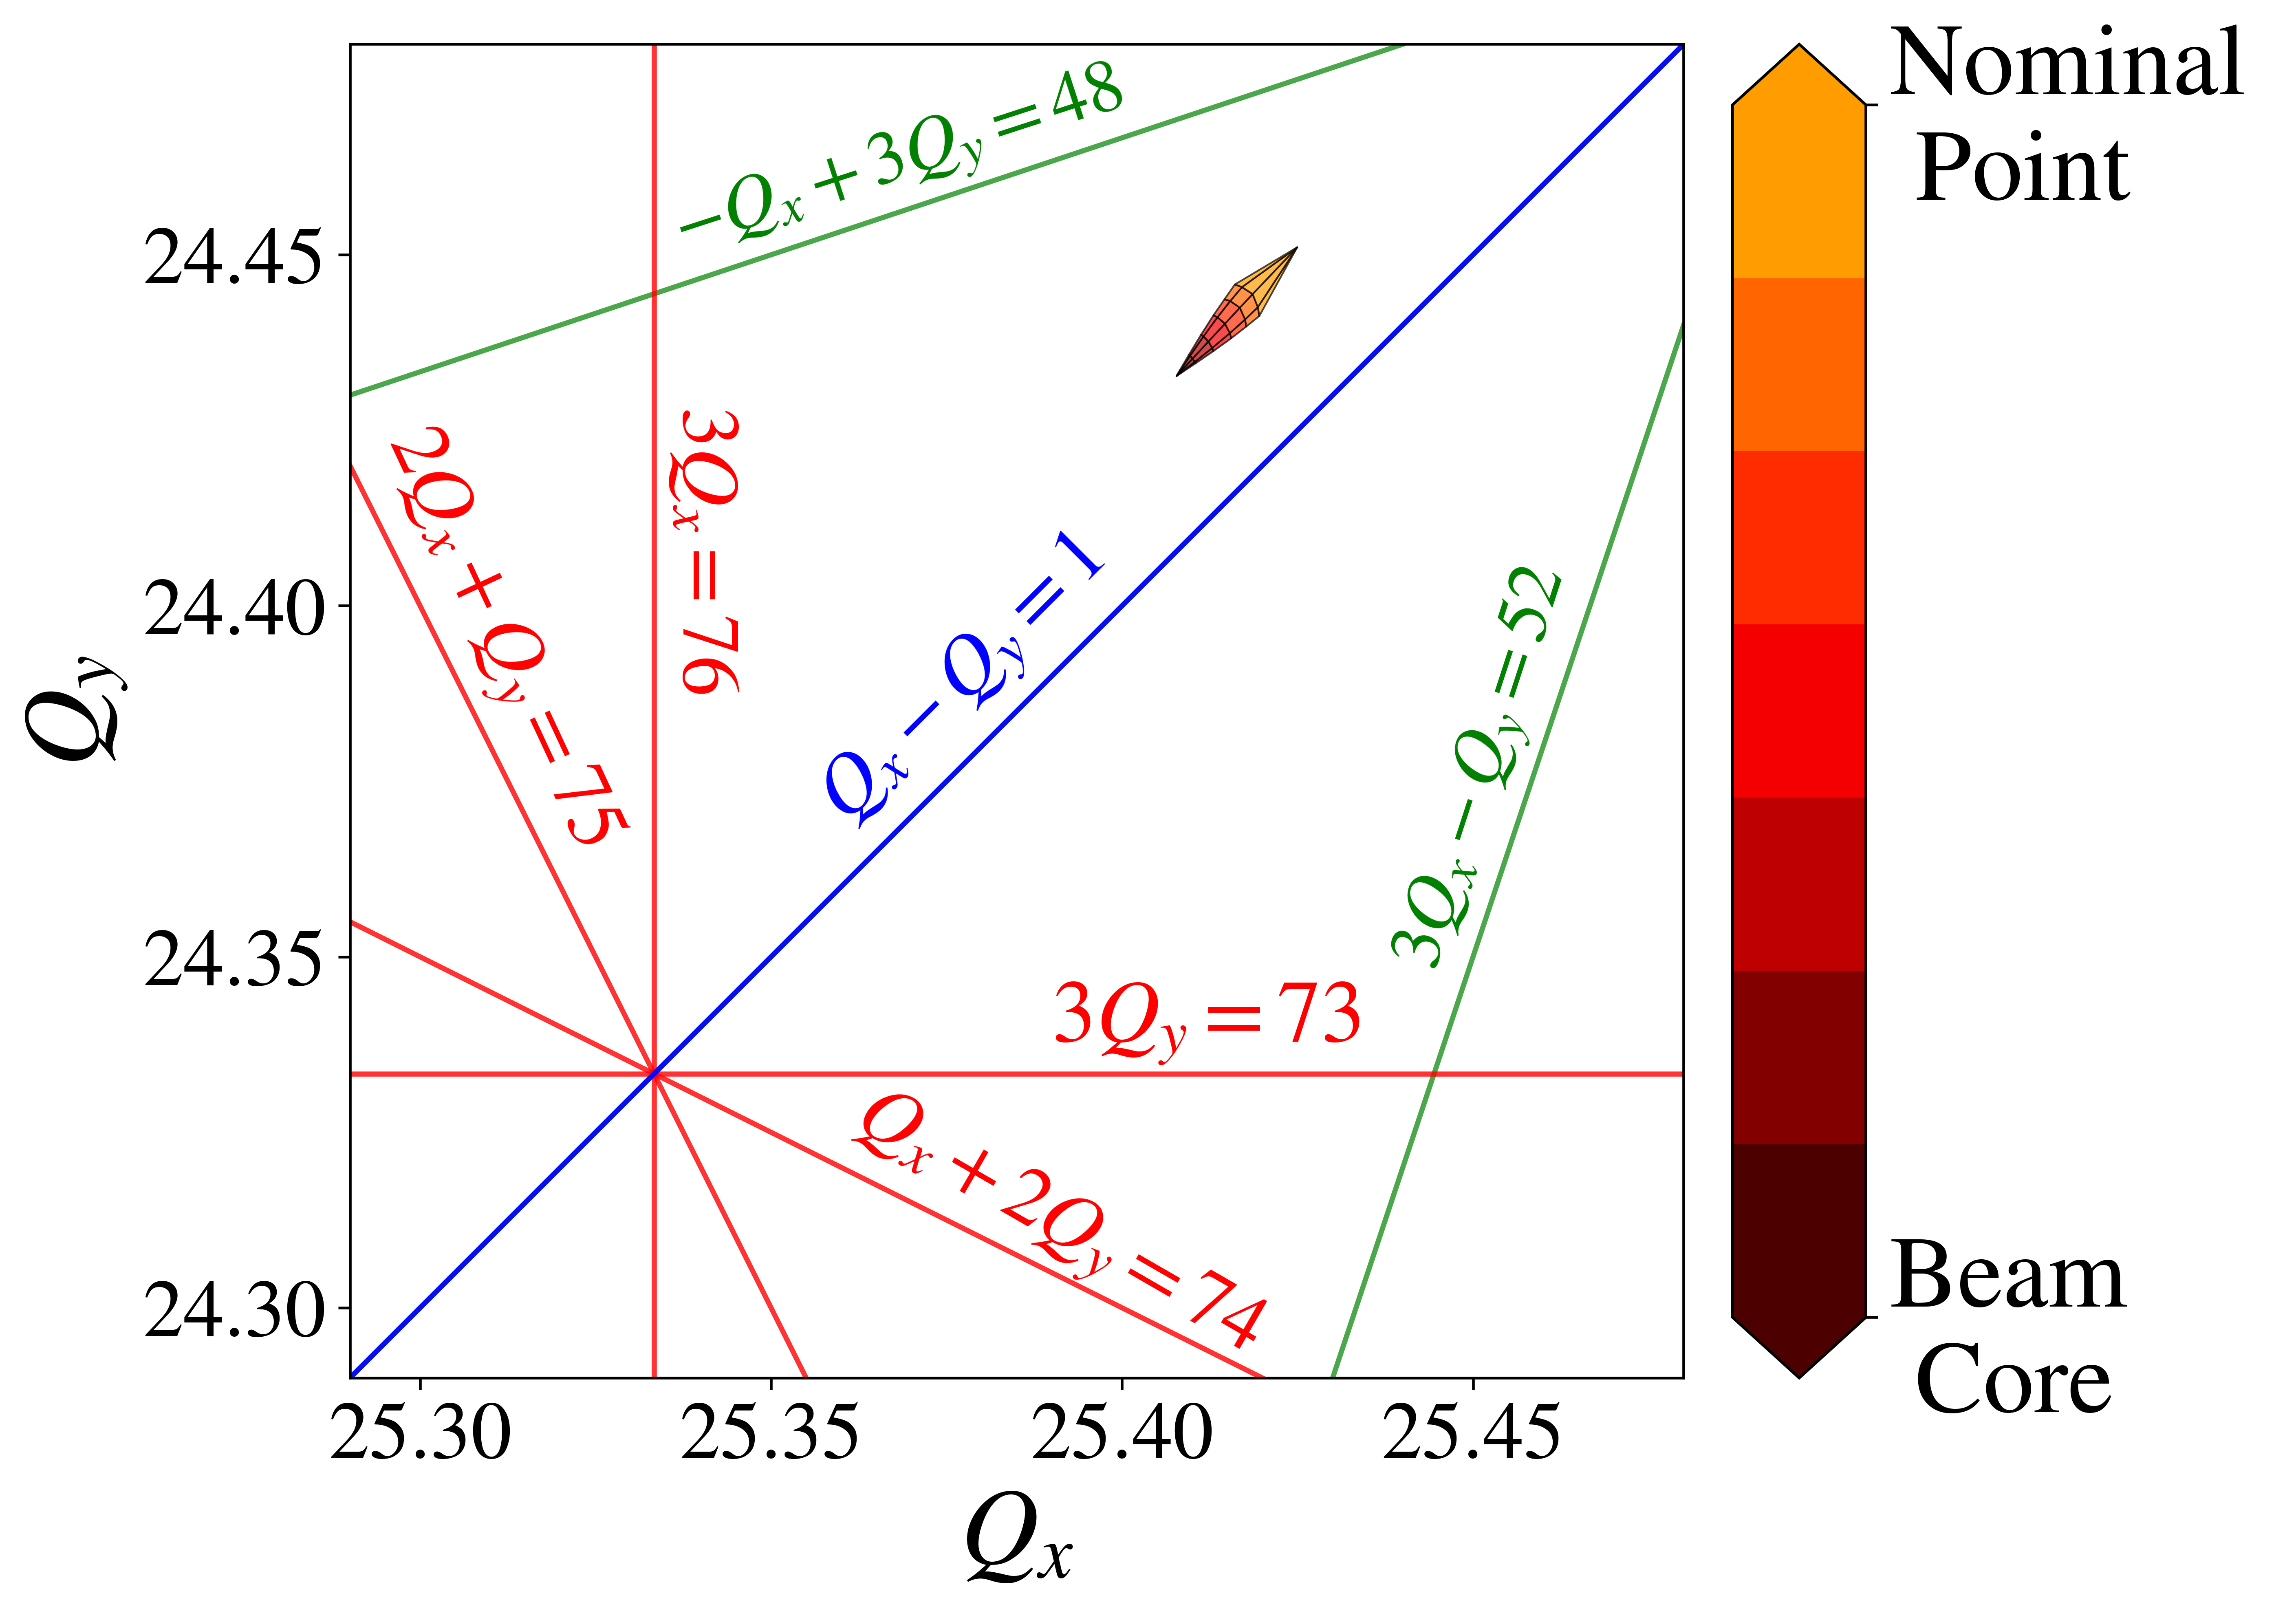
\includegraphics[width=\columnwidth]{chapter2/rrtdlow.png}
    \caption{Approximate operational tune footprint at low intensities, i.e., 1e10 particles per bunch.}
    \label{fig:rrtdlow}
 \end{figure}

\section{\label{sec:rdts}Resonance Driving Terms} 

As it turns out, the RDTs $h_{jklm}$ are related to the strength 

The resonance basis can be built by getting the quantity $h_u^{\pm}=\hat{u}\pm \hat{p_u}$ in terms of the number of turns $N$ . Specifically, for $h_x^{-}$ this reads:
\begin{multline}
    \label{eq:hx-}
    h_x^{-}(N)=\sqrt{2I_x}e^{i\left( 2\pi Q_x N +\psi_{x_0}\right)} \\
    -2i \sum_{jklm} j f_{jklm} \left( 2I_x \right)^{\frac{j+k-1}{2}}\left( 2I_y \right)^{\frac{l+m}{2}}
    e^{i \left[ \left( 1-j+k\right)\left( 2\pi Q_x N + \psi_{x_0} \right) +\left( m-l\right)\left( 2\pi Q_y N + \psi_{y_0} \right)\right]},
\end{multline}
where $Q_x$ and $Q_y$ are the horizontal and vertical tune~[3]. 

In general, RDTs are defined by the order in which they enter the one-turn normal form Hamiltonian \cite{bartolini}. The general expression to define RDTs reads:
\begin{equation}
    \label{eq:rdt1}
    h_{jklm}=\Xi _{jklm} \sum_i L_i \beta_{xi}^{\frac{j+k}{2}} \beta_{yi}^{\frac{l+m}{2}} V_{ni}e^{i\left[ (j-k)\phi_{xi} +(l-m) \phi_{yi} \right]},
\end{equation}
where $\Xi _{jklm}$ is just a constant defined as:
\begin{equation}
    \label{eq:rdt2}
    \Xi _{jklm} = -\frac{q}{p_0}\frac{1}{2^n}\frac{1}{n} {\binom{n}{l+m}} {\binom{j+k}{j}}{\binom{l+m}{l}}.
\end{equation}

For Eqs. \ref{eq:rdt1} and \ref{eq:rdt2}, $n=j+k+l+m$ represents the order of the resonance. The sum over $i$ is done over all multipoles of order $n$ and length $L_i$ that either have a normal component $V_{ni}=B_{ni}$ if $l+m$ is even, or a skew component $V_{ni}=A_{ni}$ if $l+m$ is odd. The symbols for $\beta_{xi}$, $\beta_{yi}$, $\phi_{xi}$ and $\phi_{yi}$ represent the beta functions and phase advances in each plane, respectively.

\section{\label{sec:sc1}Space Charge Tune Shift}
